% wymagania do projektu
\section{Wymagania do projektu}	
Poniżej znajduje się rysunek o numerze - \ref{rys:usecase2}. Numer został wygenerowany dynamicznie.
\begin{figure}[h!]
	\centering
	\HRule\\[1.5em]
		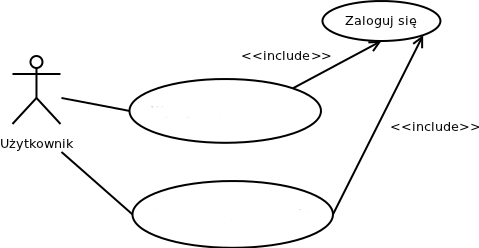
\includegraphics[width=0.5\textwidth]{img/usecase2.png}
	\\[0.3em]\HRule
	\captionof{figure}{Diagram przypadków użycia}
	\label{rys:usecase2}
\end{figure}

Mauris posuere euismod blandit. Mauris sapien ante, venenatis eget accumsan eget, lacinia at libero. Proin eget dui eros, at accumsan tortor. Aliquam sed quam libero, ac feugiat sem. Proin quis accumsan odio. Quisque posuere sollicitudin tellus, et rhoncus ipsum egestas sed. Cras nisl libero, condimentum nec porta vitae, faucibus vel purus. Pellentesque eget lorem quis elit iaculis ultricies. Fusce convallis venenatis augue, id consequat augue egestas vitae. Donec a lacus felis, consectetur tristique nibh. Sed vestibulum lectus in ipsum tincidunt fringilla. Cras sit amet consectetur nibh. Vestibulum sed est odio. 

Duis nibh enim, pretium vitae varius eget, mattis sed purus. Morbi tempor faucibus nisi at mattis. Phasellus aliquet ultrices diam, malesuada adipiscing elit iaculis quis. Fusce vel diam sit amet ligula sagittis vulputate volutpat ut dui. Maecenas cursus, turpis quis sagittis scelerisque, tortor tellus vulputate nibh, sed hendrerit nisi nisi et lacus. Suspendisse nec nisi felis. Cum sociis natoque penatibus et magnis dis parturient montes, nascetur ridiculus mus. 

Curabitur a nisi felis. Praesent tristique placerat malesuada. Nunc interdum lobortis accumsan. Lorem ipsum dolor sit amet, consectetur adipiscing elit. Nulla in sapien magna, at porttitor lorem. Vivamus condimentum convallis risus eget tincidunt. Vestibulum in condimentum magna. 

Sed quis purus est, at lobortis est. Maecenas condimentum lectus quis lectus scelerisque tristique. Sed sodales nisi in nisl tincidunt vel pretium justo hendrerit. Nullam sed ligula accumsan orci porta porttitor vitae quis lorem. Aliquam semper adipiscing tristique. Pellentesque consequat dapibus lectus vel vulputate. Proin vel ipsum massa. Vivamus suscipit, nulla ut accumsan vulputate, elit sapien hendrerit quam, at blandit odio lectus ac odio. Integer auctor, nunc vel porttitor lacinia, enim nibh faucibus nibh, a hendrerit libero dolor ut libero. 

\begin{figure}[h!]
	\centering
	\HRule\\[1.5em]
		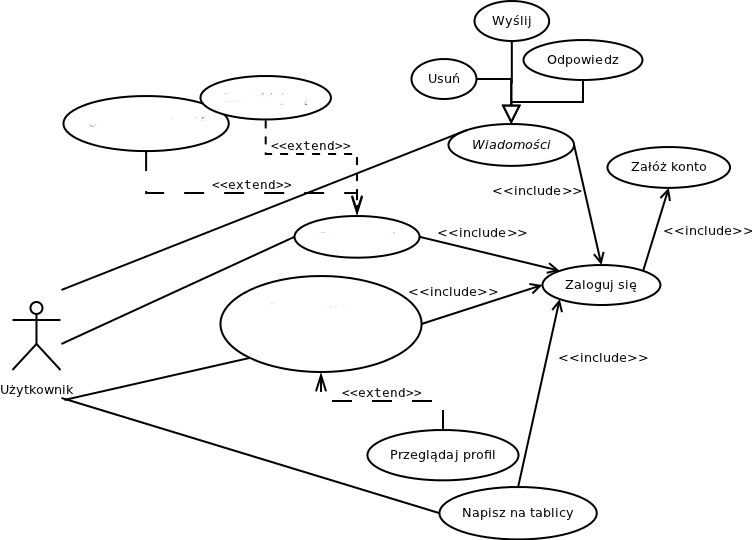
\includegraphics[width=0.8\textwidth]{img/usecase1.png}
	\\[0.3em]\HRule
	\captionof{figure}{Diagram przypadków użycia dla aplikacji internetowej}
	\label{rys:usecase1}
\end{figure}
\begin{figure}[h!]
	\centering
	\HRule\\[1.5em]
		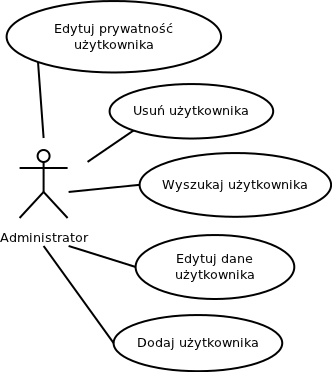
\includegraphics[width=0.4\textwidth]{img/usecase3.png}
        \\[0.3em]\HRule
	\captionof{figure}{Diagram przypadków użycia}
	\label{rys:usecase3}
\end{figure}

